\cprotect\subsection{The \verb|batch| statement}
\label{sec:eval-ast-nodes-batch}

\begin{figure}[H]
    \begin{center}
        \textbf{Diary Entry}\\[0.5em]
        ``\textit{...Finally, I added the BatchSuite which allows for batching of MethodCalls. I also updated the echo-chamber web API so that it forked multiple processes so that this feature could be tested fairly. After benchmarking a snippet of unbatched sttp code against a snippet of batched sttp code I came to the conclusion that the batch statement is quite a lot faster than if you decided against using it. The following command line output shows a fairly typical result of the testing. BenchmarkNoBatch indicates that the code snippet used does not contain the batch statement, and BenchmarkBatch indicates that the code snippet did use the batch statement. The code snippet for unbatched benchmarks was:}"
        \begin{verbatim}
            for i = 0; i < %d; i = i + 1 do
                result.result = $GET("http://127.0.0.1:3000/"; + i);
                result.results[i] = result.result.content;
                $print(result.results[i]);
            end;
            oops_forgot_this = $GET("http://127.0.0.1:3000/"; + %d);
            $print(oops_forgot_this.content);
        \end{verbatim}
        ``\textit{The code snippet for batched code is the same as the above but surrounded by the batch statement. Where `\%d' is the number of iterations to do, as indicated by the suffix on the benchmarks. The number of iterations I decided on was 10, 20, 30, 50, and 100 for both unbatched and batched benchmarks. I ran each benchmark 30 times. This is because if you let Go have free reign over the count used for benchmarks it ends with all sockets being allocated on your machine, as it runs portions of the benchmarks in parallel. The results of the benchmarks are indicated on the right-hand column in nanoseconds per operation. As you can see, the batched version of the code snippet performs quite a lot better overall. Even gaining over a 2x speed increase in the 100 iteration benchmark.}"
        \begin{verbatim}    
            $ go test -run=XXX -bench="Benchmark(No)?Batch" -benchtime=30x
            goos: darwin
            goarch: arm64
            BenchmarkNoBatch10-8    30  6713317 ns/op
            BenchmarkNoBatch20-8    30  9940293 ns/op
            BenchmarkNoBatch30-8    30  14658628 ns/op
            BenchmarkNoBatch50-8    30  19180193 ns/op 
            BenchmarkNoBatch100-8   30  35917022 ns/op
            BenchmarkBatch10-8      30  4455203 ns/op
            BenchmarkBatch20-8      30  5903021 ns/op
            BenchmarkBatch30-8      30  6921599 ns/op
            BenchmarkBatch50-8      30  9529031 ns/op
            BenchmarkBatch100-8     30  15955876 ns/op
        \end{verbatim}
        \tiny{2:17 am on November 20, 2021}
    \end{center}
\end{figure}

One of the main motivations for creating \verb|sttp| was to enable the programmer to easily `batch' multiple HTTP requests and execute them concurrently. This is a technique that I use often whilst requesting information from web servers that don't enforce a strict rate limit. Dispatching a `batch' of HTTP requests to multiple worker threads is often always faster than executing each HTTP request sequentially (from personal experience). In \verb|sttp| the \verb|batch| statement was implemented for this very reason.

\begin{verbatim}
batch this
    for i = 0; i < 100; i = i + 1 do
        result.result = $GET("http://127.0.0.1:3000/" + i);
        result.results[i] = result.result.content;
        $print(result.results[i]);
    end;
    oops_forgot_this = $GET("http://127.0.0.1:3000/" + 100);
    $print(oops_forgot_this.content);
end;
\end{verbatim}

The \verb|batch| statement can wrap any \verb|Block| of code. It executes the wrapped code in two passes:

\begin{enumerate}
    \item Batching each instance of the \verb|MethodCall| AST node. Then executing these batched HTTP requests in several worker goroutines, adding the result of each to a result queue.
    \item Executing the inner \verb|Block| again, and replacing each instance of the \verb|MethodCall| AST node with the next result from the result queue.
\end{enumerate}

A more in-depth explanation of these steps is explained within the \hyperref[sec:batching]{specification}. The data-structure used to achieve this is the \verb|BatchSuite| type. This stores a list of jobs in the order that the \verb|MethodCall|s were encountered during the execution of the first pass. Along with this list, there is a counter for current ID to use for the next enqueued job, as well as a pointer back to the \verb|Batch| AST node. This work is then executed using a pool of goroutines, the number of which is decided by the number of incoming jobs.

\inputminted[firstline=72, lastline=78, autogobble, breaklines, tabsize=4]{go}{../../src/batch.go}

\inputminted[firstline=89, lastline=102, autogobble, breaklines, tabsize=4]{go}{../../src/batch.go}

\inputminted[firstline=124, lastline=160, autogobble, breaklines, tabsize=4]{go}{../../src/batch.go}

Here, the \verb|methodWorker| function acts as a worker `thread' which takes a readable channel (\mintinline{go}{<-chan}) of jobs as well as a writeable channel (\mintinline{go}{chan<-}) of results. This worker function is then spawned off \verb|min(MaxWorkers, numJobs)| times (where \verb|MaxWorkers = 20|). The jobs within \verb|BatchSuite.Batch| are then enqueued in the jobs queue. We then read from the results queue into a \verb|BatchResults| instance. \verb|BatchResults| implements \verb|heap.Interface| so the complexity of this operation is: $O(n \log n)$. This \verb|BatchResults| queue's reference will be stored within the \verb|VM|, and will act as the main way of checking whether the batch is currently in its second pass.

\begin{verbatim}
// Example 1: A batch statement within a batch statement.
batch this
    a.result = $GET("http://127.0.0.1:3000/hello/world");
    batch this
        uh.oh = $GET("http://127.0.0.1:3000/uh/oh");
    end;
end;

// Example 2: A batch statement with no method calls.
batch this
    $print("no method calls in 'ere");
end;

// Example 3: MethodCall pointer mismatch.
batch this
    x = $GET("http://127.0.0.1:3000/the/flow/depends/on/this/request");
    y = $GET("http://127.0.0.1:3000/the/flow/depends/on/this/request/also");
    if x.code == 200 && y.code == 200 then
        wont_be_batched = $GET("http://127.0.0.1:3000/wont/be/batched");
    end;
    uh_oh = $GET("http://127.0.0.1:3000/uh/oh");
end;

// Example 4: No more results left in the results queue.
batch this
    x = $GET("http://127.0.0.1:3000/the/flow/depends/on/this/request");
    y = $GET("http://127.0.0.1:3000/the/flow/depends/on/this/request/also");
    if x.code == 200 && y.code == 200 then
        wont_be_batched = $GET("http://127.0.0.1:3000/wont/be/batched");
    end;
end;

// Example 5: Too many results left after executing batch.
batch this
    x = $GET("http://127.0.0.1:3000/the/flow/depends/on/this/request");
    if x.code != 200 then
        wont_be_batched = $GET("http://127.0.0.1:3000/will/be/batched");
    end;
end;
\end{verbatim}

The \verb|batch| statement has a few edge cases that need to be handled due to the semantics of the operation. Consider the above \verb|sttp| code, all examples above will return an error (that can be caught).

\textbf{Example 1}: \verb|batch| statements do not support another \verb|batch| statement within them. This is because this behaviour is undefined (for the moment). This is implemented by simply checking if there is a \verb|BatchSuite| or \verb|BatchResults| available in the \verb|VM| when evaluating each \verb|Batch| AST node.

\textbf{Example 2}: a \verb|batch| statement with no \verb|MethodCall|s within it, only has its first-pass executed. This is accomplished by first caching the \verb|VM|'s stdout and stderr then setting them to temporary buffers within memory. If after the first pass no \verb|MethodCall|s have been batched, the temporary buffers will be written to the cached stdout and stderr which will then be set back to be the \verb|VM|'s stdout and stderr. The batch is then aborted.

\textbf{Example 3}: in this example the \verb|MethodCall| that is being stored in the \verb|wont_be_batched| variable is not batched during the first pass. This is because the value of \verb|x| and \verb|y| will be set to \verb|null| during the first pass, as this is what is returned by all \verb|MethodCall|s within the first pass. Therefore, the \verb|MethodCall| within the \verb|if| statement will not be batched, but the one after it will be. However, when in the second pass, the \verb|MethodCall| within this \verb|if| statement will be evaluated, and the next result from the batch will be dequeued. Results within the results queue store a pointer back to the original \verb|MethodCall| that was enqueued as a job. This pointer can then be compared to the \verb|MethodCall| that is currently being evaluated. If it doesn't match, then an error will be thrown.

\textbf{Example 4}: Similar to \textbf{Example 3}, this snippet will not batch the \verb|MethodCall| within the \verb|if| statement. However, this time there is no \verb|MethodCall| following the \verb|if|. This results in there being no result left to dequeue when in the second pass and evaluating the \verb|MethodCall| within the \verb|if|.

\textbf{Example 5}: Similar to \textbf{Example 3} and \textbf{Example 4}. However, this snippet will \textbf{not} batch the \verb|MethodCall| within the \verb|if| statement, and will not be evaluated in the second pass. This results in there being one more result in the results queue at the end of the \verb|batch| statement. In these cases, we are able to continue execution normally, but for completeness we raise an error.

\subsubsection{Updating the echo-chamber test web API}

In order to give a fair analysis of the performance of batching, the echo-chamber test web API server that I wrote as a test program will need to be modified so that it can serve multiple requests. In nodejs this was fairly easy to implement by forking the web server process into multiple worker processes that share the same socket. This has the effect of acting as a rudimentary load-balancer, allowing multiple inbound requests to be a handled at once.

\subsubsection{Performance}

\verb|batch| statements need to be performant in order to be more useful than just executing \verb|MethodCall|s synchronously. When developing the \verb|batch| statement there was some apprehension to how performant the execution of two passes of the \verb|Block| within a \verb|batch| statement would be. This is because there is effectively double the overhead. To benchmark the performance of the \verb|batch| statement I wrote the following \verb|sttp| code snippet:

\begin{figure}[H]
    \begin{verbatim}
for i = 0; i < %d; i = i + 1 do
    result.result = $GET("http://127.0.0.1:3000/"; + i);
    result.results[i] = result.result.content;
    $print(result.results[i]);
end;
oops_forgot_this = $GET("http://127.0.0.1:3000/"; + %d);
$print(oops_forgot_this.content);
    \end{verbatim}
    \cprotect\caption{Code snippet used for benchmarking synchronous \verb|MethodCall|s. The concurrent version of this snippet is just wrapped with a \verb|batch| statement.}
    \label{sec:eval-ast-nodes-batch-bench-snippet}
\end{figure}

I then wrote multiple Go benchmarking functions within \verb|src/main_test.go| that used \verb|Sprintf| to replace \verb|%d| with: 10, 20, 30, 50, 100, and 200 to test the performance of evaluating \verb|MethodCall|s synchronously. I then replicated this for benchmarking the \verb|batch|ed concurrent code by wrapping the code snippet within a \verb|batch| statement. This gave me six benchmarks for a control, as well as six benchmarks for the concurrent code. Two important things to note about the benchmarking that took place:

\begin{enumerate}
    \item Due to the large numbers of socket descriptors that need to be open on the benchmarking machine, I had to increase the limit of the number of open socket descriptors to run the benchmarks successfully (on Unix based systems this can be done via the \verb|ulimit| command). A possible aggravator of this is that Go runs each iteration of each benchmarking function in parallel. Thus increasing the overall number of socket descriptors used by a factor of the number of iterations to execute.
    \item The time to generate the parser as well as parse the input snippet are \textbf{not} taken into account when timing each iteration.
\end{enumerate}

\label{sec:eval-ast-nodes-batch-bench-1-intro}
The first benchmarks I ran only used 10, 20, 30, 50, and 100 as the number of iterations and were executed 30 times each. These iterations are then averaged giving an average execution time per benchmarking function. Below shows the results of this first execution:

\begin{center}
    Command that was used to run benchmarks:\\[0.5em]
    \verb|go test -run=XXX -bench="Benchmark(No)?Batch" -benchtime=30x|
\end{center}

\begin{figure}[H]
    \centering
    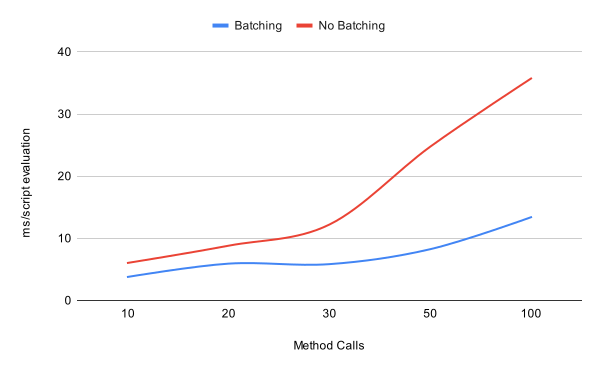
\includegraphics{../specification_for_language/assets/batching-chart-100-calls.pdf}
    \cprotect\caption{Graph showing the average number of milliseconds taken to run the \verb|sttp| script shown \hyperref[sec:eval-ast-nodes-batch-bench-snippet]{above} when \verb|%d| is set to 10, 20, 30, 50, and 100, after running the script 30 times for each \verb|%d|.}
    \label{sec:eval-ast-nodes-batch-bench-1-graph}
\end{figure}

The graph above shows that when executing up to 20 HTTP method calls within a batch statement, there is a smaller performance increase over executing outside a batch statement, than when executing over 20 HTTP method calls.

\label{sec:eval-ast-nodes-batch-bench-2-intro}

The next benchmarks I ran used 10, 20, 30, 50, and 200 as the number \verb|%d| was formatted with. The number of iterations to average each benchmarking function with dropped down to 15. This was due to socket limitations. Below shows the results of this second execution:

\begin{center}
    Command that was used to run benchmarks:\\[0.5em]
    \verb|go test -run=XXX -bench="Benchmark(No)?Batch" -benchtime=5x -cpu=8 -count=3|
\end{center}

\begin{figure}[H]
    \centering
    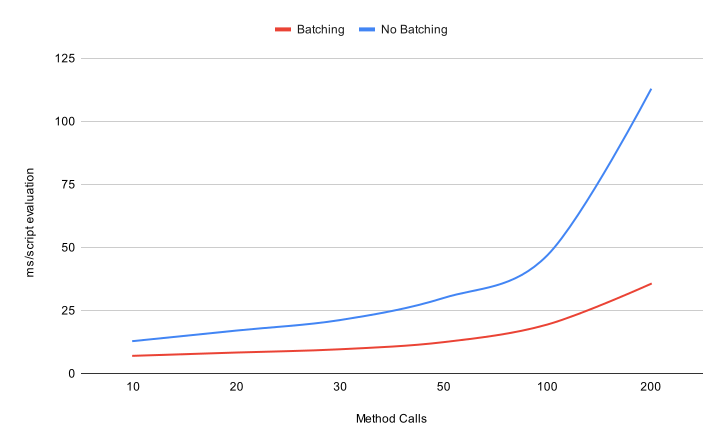
\includegraphics[scale=0.75]{../specification_for_language/assets/batching-chart-200-calls.pdf}
    \cprotect\caption{Graph showing the average number of milliseconds taken to run the \verb|sttp| script shown \hyperref[sec:eval-ast-nodes-batch-bench-snippet]{above} when \verb|%d| is set to 10, 20, 30, 50, 100, and 200, after running the script $5 * 3$ times for each \verb|%d|.}
    \label{sec:eval-ast-nodes-batch-bench-2-graph}
\end{figure}

The graph above shows a similar result to that of the \hyperref[sec:eval-ast-nodes-batch-bench-1-intro]{previous benchmark}, but also shows that the growth rate of the milliseconds that it takes to run the test script is a lot less severe when using batching then when not using it at all.

\cprotect\textbf{Why is the speed increase greater when parallelising a lot of \verb|MethodCall|s, than parallelising fewer \verb|MethodCall|s?}